% !TEX TS-program = pdflatex
% !TEX encoding = UTF-8 Unicode

% This file is a template using the "beamer" package to create slides for a talk or presentation
% - Talk at a conference/colloquium.
% - Talk length is about 20min.
% - Style is ornate.

% MODIFIED by Jonathan Kew, 2008-07-06
% The header comments and encoding in this file were modified for inclusion with TeXworks.
% The content is otherwise unchanged from the original distributed with the beamer package.

\documentclass{beamer}


% Copyright 2004 by Till Tantau <tantau@users.sourceforge.net>.
%
% In principle, this file can be redistributed and/or modified under
% the terms of the GNU Public License, version 2.
%
% However, this file is supposed to be a template to be modified
% for your own needs. For this reason, if you use this file as a
% template and not specifically distribute it as part of a another
% package/program, I grant the extra permission to freely copy and
% modify this file as you see fit and even to delete this copyright
% notice. 


\mode<presentation>
{
  \usetheme{Warsaw}
  % or ...

  \setbeamercovered{transparent}
  % or whatever (possibly just delete it)
}


\usepackage[english]{babel}
% or whatever

\usepackage[utf8]{inputenc}
% or whatever

\usepackage{times}
\usepackage[T1]{fontenc}
% Or whatever. Note that the encoding and the font should match. If T1
% does not look nice, try deleting the line with the fontenc.
 \newcommand{\abs}[1]{\left|{#1}\right|}
 \newcommand{\av}[1]{\left\langle #1 \right\rangle}
 
  \newcommand{\br}[1]{\langle #1|}
  \newcommand{\ke}[1]{|#1\rangle}
  \newcommand{\bk}[2]{\langle #1|#2\rangle}
  \newcommand{\kb}[2]{\ke{#1}\br{#2}}
  \newcommand{\var}[2]{\langle #1|#2\rangle} 
  \newcommand{\ov}[2]{\abs{\var{#1}{#2}}^2}
\newcommand{\td}[1]{\widetilde{#1}}

%\title[Short Paper Title] % (optional, use only with long paper titles)
%{Second Examination}

\title
{Optimal Measurements}

\author[Vadim Yerokhin] % (optional, use only with lots of authors)
{Vadim Yerokhin }
% - Give the names in the same order as the appear in the paper.
% - Use the \inst{?} command only if the authors have different
%   affiliation.

% - Use the \inst command only if there are several affiliations.
% - Keep it simple, no one is interested in your street address.

\date[CFP 2003] % (optional, should be abbreviation of conference name)
{Hunter College, November 18th 2013 }
% - Either use conference name or its abbreviation.
% - Not really informative to the audience, more for people (including
%   yourself) who are reading the slides online


% If you have a file called "university-logo-filename.xxx", where xxx
% is a graphic format that can be processed by latex or pdflatex,
% resp., then you can add a logo as follows:

% \pgfdeclareimage[height=0.5cm]{university-logo}{university-logo-filename}
% \logo{\pgfuseimage{university-logo}}



% Delete this, if you do not want the table of contents to pop up at
% the beginning of each subsection:
\AtBeginSubsection[]
{
  \begin{frame}<beamer>{Outline}
    \tableofcontents[currentsection,currentsubsection]
  \end{frame}
}


% If you wish to uncover everything in a step-wise fashion, uncomment
% the following command: 

%\beamerdefaultoverlayspecification{<+->}


\begin{document}

\begin{frame}
  \titlepage
\end{frame}

\begin{frame}{Outline}
  \tableofcontents[pausesections]
  % You might wish to add the option [pausesections]
\end{frame}


% Structuring a talk is a difficult task and the following structure
% may not be suitable. Here are some rules that apply for this
% solution: 

% - Exactly two or three sections (other than the summary).
% - At *most* three subsections per section.
% - Talk about 30s to 2min per frame. So there should be between about
%   15 and 30 frames, all told.

% - A conference audience is likely to know very little of what you
%   are going to talk about. So *simplify*!
% - In a 20min talk, getting the main ideas across is hard
%   enough. Leave out details, even if it means being less precise than
%   you think necessary.
% - If you omit details that are vital to the proof/implementation,
%   just say so once. Everybody will be happy with that.


\section{Introduction}
\subsection{Why Measurement Theory?}
\begin{frame}
\begin{itemize}
\item
Classical bits versus quantum bits: instead of just a 0 or 1, quantum bits can maintain a superposition state
\pause
\item
The probabalistic nature of detection: only orthogonal states can be discriminated perfectly
\pause
\item
Quantum Computing
\pause
\item
Quantum Communication
\end{itemize}
\end{frame}
\subsection{Our Game}
\begin{frame}
\begin{itemize}
\item
Someone prepares one two different pure states $\ke {\psi_i} = \alpha_i \ke 0 +  \beta_i \ke 1$
\pause
\item
Each state has a different likelihood $\eta_i$
\pause
\item
One particle (state) is sent at a time.  Our job is to guess as best we can what state was sent.
\pause
\item
The particle can be sent through one channel, or fiber optic cable.  It could be sent over many cables, or the cables could be noisy.
\end{itemize}

\end{frame}
\subsection{The Math of Measurement Theory}

\begin{frame}{Density Matrices}
  % - A title should summarize the slide in an understandable fashion
  %   for anyone how does not follow everything on the slide itself.
A density matrix is a generalized state that is a statistical collection of pure states defined by four properties:
  \begin{itemize}


\item   
1. $\rho  = \sum_i \eta_i \kb{\psi_ i}{\psi_i}$ where $\sum \eta_i = 1$
\pause
\item

2. It is Hermitian 
\pause
\item

3.  $Tr \rho = 1$
\pause
\item
4. $\br {\phi_i} \rho \ke {\phi_i} \geq 0$
\end{itemize}
\end{frame}
\begin{frame}{Measurement Operators}
\begin{itemize}
\item
Measurements are a decomposition of the identity in terms of positive semi-definite matrices.
\pause
 \item
    A measurement can be either a projector or a generalized measurement.  In the latter case it must fulfill only 2 properties:
\pause

           1.  $\sum \Pi_i = 1$
\pause

	2. They are Hermitian.  This corresponds to real eigenvalues (measurement outcomes).


	
  \end{itemize}
\end{frame}

\begin{frame}{Expectation Values as Traces}
Since non-orthogonal states cannot be discriminated perfectly, we can speak of the probability of a given outcome:

\begin{itemize}

\item
	$\av {\Pi_i} = \sum_j \eta_j \br {\psi_j} \Pi_i \ke {\psi_j} = Tr(\Pi_i \rho)$

\end{itemize}
\end{frame}
\subsection{Discrimination Strategies}
\begin{frame}{Minimum Error Discrimination}
	The first measurement strategy was Minimum Error Discrimination.

\begin{itemize}
\item
	Two orthogonal projectors, each clicks for a state.
\pause
\item
	There is a success rate and an error rate if the states are not orthogonal.

\[ P_s =\eta_1 Tr(\rho_1 \Pi_1) + \eta_2Tr(\rho_2 \Pi_2)\]
\[ P_e = \eta_2 Tr(\rho_2 \Pi_1) +\eta_1 Tr(\rho_1 \Pi_2)\]
\pause
\item
	The minimum error rate for pure states is achieved by the Helstrom bound.

\[P_E = \frac{1}{2}(1- \sqrt{1-4 \eta_1 \eta_2 \ov{\psi_1}{\psi_2}})\]
\end{itemize}
\end{frame}
\begin{frame}{Minimum Error Graph}
\begin{figure}[th]
\centering
$%
\begin{array}{c}
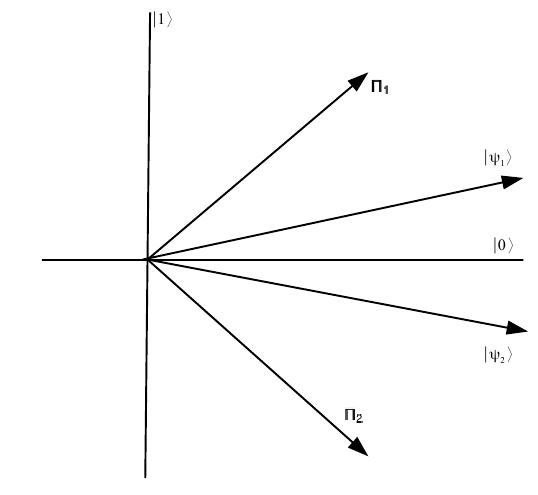
\includegraphics[height=7 cm]{ME.png} \\

\end{array}%
$%

\label{fig:Graphs}
\end{figure}
\end{frame}
\begin{frame}{Unambigious State Discrimination}



\begin{itemize}
\pause
\item
	Make the measurement operators orthogonal to the state that we don't want to measure.
\pause
\item
	Since they are no longer orthogonal they don't sum to the identity. A third, inconclusive outcome is necessary.
\item
	The detector corresponding to the inconclusive outcome we call $\Pi_0$
\pause

\item
	The failure probability we call Q:

\[Q =  \eta_1 Tr(\rho_1 \Pi_0) +\eta_2  Tr(\rho_2 \Pi_0) = Tr(\rho \Pi_0)\]
\pause
\item
$ Q_0 = 2 \sqrt{\eta_1\eta_2} cos \theta$  is the failure rate that corresponds to the best measurement.
\end{itemize}

\end{frame}
\begin{frame}{Unambiguous State Discrimination Graph}
\begin{figure}[th]
\centering
$%
\begin{array}{c}
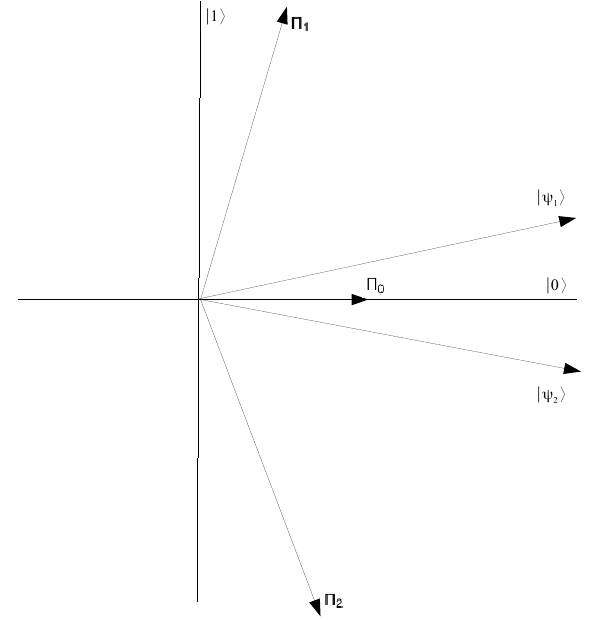
\includegraphics[height=7 cm]{UD.png} \\

\end{array}%
$%

\label{fig:Graphs}
\end{figure}
\end{frame}
\begin{frame}{Intermediate Measurement Transformation}
The Intermediate Measurement scheme interpolates optimally between ME and UD. The transformation we want takes us from 3 detection operators down to two:

\[\Pi_1 + \Pi_2 + \Pi_0 = I\]
 \[\Omega ^{-1/2}[\Pi_1 + \Pi_2] \Omega^{-1/2}=\widetilde \Pi_{1} + \widetilde \Pi_{2} = I\] 

where $\Omega = I - \Pi_0$

\end{frame}
\begin{frame}{Intermediate Measurement Optimization}
The transformation changes the density matrices and a-priori probabilities, which formulate a new ME problem.  The solution is a Helstrom bound in which a further optimization is required.  The final result is:

\[ P_e = \frac{1}{2} (1 - Q -\sqrt{(1-Q)^2 - (Q-Q_0)^2})\]
\[\]
$0\leq Q \leq Q_0$  where $ Q_0 = 2 \sqrt{\eta_1\eta_2} cos \theta$
\end{frame}

\section{Subspace Measurements}

\subsection{Two Subspaces}

\begin{frame}{Two Subspaces Setup}

We consider the case of two mixed states that form two two-dimensional Hilbert spaces. Hence our density matrices are in four dimensions consisting of two tensor product spaces:
\[ \rho_1 = r_1 \vert r_1 \rangle \langle r_1 \vert  + r_2 \vert r_2 \rangle \langle r_2 \vert\]
\[ \rho_2 = s_1 \vert s_1 \rangle \langle s_1 \vert  + s_2 \vert s_2 \rangle \langle s_2 \vert\]

With our full density matrix is $ \rho = \eta_1 \rho_1 + \eta_2 \rho_2$

We begin by focusing on the first subspace and define our measurement operators for the first subspace as

\[ \widetilde \Pi_{1,1} + \widetilde \Pi_{2,1} = I_1\]

Where $I_1$ is the identity matrix of the first subspace
\end{frame}
\begin{frame}
We define $\Pi_{0,1} = \xi_1 \ke 0_{11} \br 0 $and we find the failure rate to be

\[ Q_1 = \xi_1 [ \eta_{1,1} cos^2 \phi_1 + \eta_{2,1} cos^2 (\theta_1 - \phi_1)]\]

Where $\theta_1 $ is the overlap angle between the two states in subspace 1 , $\phi_1$ is the angle $\ke {r_1}$ makes with respect to $\vert 0 \rangle_1$ , and $\eta_{1,i} = \eta_1 r_i$  , $\eta_{2,i} = \eta_2 s_i$

\end{frame}
\begin{frame}
The error rate in that subspace is

\[P_{e,1} = \eta_{1,1} \langle r_1 \vert \Pi_{2,1} \vert r_1 \rangle + \eta_{2,1} \langle s_1 \vert \Pi_{1,1} \vert s_1 \rangle \]

We introduce the normalized state vector \[ \vert \widetilde{r_1} \rangle  = \frac{ \Omega^{1/2} \vert r_1 \rangle}{\sqrt{\langle r_1 \vert \Omega \vert r_1 \rangle}} \]
and normalized coefficients

\[ \widetilde{\eta_{1,1}} = \frac{\eta_{1,1} \langle r_1 \vert \Omega \vert r_1 \rangle}{\eta_{1,1} \langle r_1 \vert \Omega \vert r_1 \rangle + \eta_{2,1} \langle s_1 \vert \Omega \vert s_1 \rangle}\]
\end{frame}

\begin{frame}
We get

\[P_{e,1} = \eta_{1,1} \langle r_1 \vert \Omega \vert r_1 \rangle \langle \widetilde{r_1} \vert \widetilde{\Pi_2} \vert \widetilde{r_1} \rangle + \eta_{2,1} \langle s_1 \vert \Omega \vert s_1 \rangle \langle \widetilde{s_1} \vert \widetilde{\Pi_1} \vert \widetilde{s_1}\rangle \]
$=$
\[  [\eta_{1.1} \langle r_1 \vert \Omega \vert r_1 \rangle + \eta_{2,1}\langle s_1 \vert \Omega \vert s_1 \rangle](\widetilde{\eta_{1,1}}\langle\widetilde{r_1} \vert \widetilde{\Pi_2} \vert \widetilde{r_1} \rangle + \widetilde{\eta_{2,1}} \langle \widetilde{s_1} \vert \widetilde{\Pi_1} \vert \widetilde{s_1}\rangle )\]

We notice that the second set of ( ) with all tildes contains a pure state minimum error problem, while with the notation $ \eta_{1,1} +\eta_{2,1} = \omega_1$ the left hand set of [ ]  can be reworked into $\omega_1 - Q_1 $

\[ = \frac{1}{2} [\omega_1 - Q_1] (1- \sqrt{1 - 4 \widetilde{\eta_{1,1}} \widetilde{\eta_{2,1}} \vert \langle \widetilde{r_1} \vert \widetilde{s_1} \rangle \vert ^2 }) \] 
\end{frame}

\begin{frame}

\[P_{e,1} = \frac{1}{2} ( \omega_1 - Q_1 - \sqrt{ ( \omega_1 - Q_1)^2 -(Q_{0,1} - Q_1 sin 2 \phi )^2})\]

where we used the notation $Q_{0,1} = 2 \sqrt{\eta_{1,1}\eta_{2,1}} cos \theta_1$ and 

 $ sin \phi = \frac{ \sqrt {\eta_{2,1}} cos (\theta_1 - \phi_1)}{\sqrt{ \eta_{1,1} cos^2 (\phi_1)+ \eta_{2,1} cos^2 (\theta_1 - \phi_1)}}$

Minimization on the expression as a function of $\phi$ tells us to set $\phi =\frac{\pi}{4}$ so finally

\[P_{e,1} = \frac{1}{2} ( \omega_1 - Q_1 - \sqrt{ ( \omega_1 - Q_1)^2 -(Q_{0,1} - Q_1 )^2})\]
\end{frame}
\begin{frame}

This result agrees with the single subspace limit and in fact is simply the optimized solution for that subspace alone. We can derive a similar result for the other subspace, so are now ready to consider an optimal distribution of failure among the two subspaces.  We want to treat this distribution problem for N subspaces so we first generalize our preceding solution to 2n dimensions.
\end{frame}

\subsection{General Solution}

\begin{frame}{Normalization}

We want to generalize the formalisim to 2n dimensions.   Recognizing the measurement probabilities in each subspace don't add up to 1, we want to normalize the new operators so that we can solve them like the 2d case where we had
\[P_e+ P_s+ Q= 1\]

Instead, now we have
\[P_{e,i} + P_{s,i} + Q_i = \eta_{1,i} + \eta_{2,i} = \omega_i\]

Where we call $P_{e,i}$ the probability of error in subspace $i$ and $P_{s,i}$, $Q_i$ the success and the failure probabilities in that subspace too.  And $\omega_i$ is the weight of that subspace, or the total probabilitiy of a partilcle being found therein.

\end{frame}
\begin{frame}

So we redefefine
\[ \bar{P_{e,i}} +\bar{P_{s,i}} + \bar{Q_i} = 1 \]

with $ \bar{\bullet} = \frac{\bullet}{\omega_i} $

We redefine the weights $\bar{\eta_{1,i}} = \frac{\eta_1 r_i}{  \omega_i }$ and $ \bar{\eta_{2,i}} = \frac{ \eta_2 s_i }{\omega_i}$ that still sum 1, so that the states and measurements don't change.
\end{frame}
\begin{frame}

Now it is straightforward to apply the result of the renormalized minimization to each subspace: 

namely,
 \[\bar{P_{e,i}} = \frac{1}{2}( 1-\bar{Q_i} - \sqrt{(1-\bar{Q_i})^2 - (\bar{Q_{0,i}} -\bar{ Q_i})^2})\] where 
\[\bar{Q_{0,i}} = 2 \sqrt{\bar{\eta_{1,i}}\bar{\eta_{2,i}}}cos\theta_i\]

is also

\[P_{e,i}= \frac{1}{2}( \omega_i-Q_i - \sqrt{(\omega_i-Q_i)^2 - (Q_{0,i} - Q_i)^2})\]
\end{frame}

\begin{frame}{Lagrangian Optimization}


Since each subspace can vary independently we are interested in the optimal values for $Q_i$ as a function of fixed $Q$

If we consider this a Lagrange Multiplier problem with $P_{e,i}$ with constraint $\sum Q_i = Q$ then we get the constrained function

\[F = P_{e,i} - \lambda (\sum Q_i - Q)\]

\[ =\frac{1}{2}( \omega_i-Q_i - \sqrt{(\omega_i - Q_{0,i}) (\omega_i + Q_{0,i} -2 Q_i)}  - \lambda (\sum Q_i - Q)\]
\end{frame}
\begin{frame}
\[\frac{d F}{d Q_i} =0 \]

when

\[Q_i = \frac{1}{2}( \omega_i + Q_{0,i} - \frac{\omega_i - Q_{0,i}}{(2\lambda +1)^2})\]

Since $\sum Q_i = Q$ we have
\[ Q= \sum Q_i = \frac{1}{2}( 1 + Q_0 - \frac{1 - Q_0}{(2\lambda +1)^2})\]  where $Q_0 = \sum Q_{0,i} = 2 \sqrt{\eta_1 \eta_2} \sum \sqrt{r_i s_i}cos \theta_i$
\end{frame}
\begin{frame}
Solving for $\lambda$ we find
\[\frac{2Q - 1 - Q_0}{1-Q_0} = \frac{-1}{(2\lambda+1)^2}\] 

We insert this expression for $\lambda$ into the expression for $Q_i$ to eliminate the Lagrange Multiplier, and find its optimal value as
\[Q_i = \frac{1}{2}( \omega_i + Q_{0,i} + (\omega_i - Q_{0,i})(\frac{2Q - 1 - Q_0}{1-Q_0}))\]


Now the optimized subspace error rate is

 \[P_{e,i}= \frac{1}{2}( \omega_i-Q_i - (\omega_i - Q_{0,i})\sqrt{\frac{1+ Q_0 -2 Q}{1-Q_0}})\]

with the total optimal error rate $P_e = \sum P_{e,i}$
\[P_e = \frac{1}{2}(1-Q-\sqrt{(1-Q)^2-(Q-Q_0)^2})\]
\end{frame}

\begin{frame}{Threshold Structure}
The range of the subspace solution is valid strictly for more than one subspace and is limited by the positivity of $Q_i$.
If we re-write it as

\[ Q_i = \frac{Q_{0,i} - \omega_i Q_0 + Q(\omega_i - Q_{0,i})}{1- Q_0}\] and set it to zero we find the critical value of Q for that subspace to be

\[Q= Q^i_c = \frac {\omega_i Q_0 - Q_{0,i}}{\omega_i- Q_{0,i}}\] 

So when Q falls below $Q^j_c$ we fix $Q_j = 0$ and discard that subspace from our optimization. 
\end{frame}
\begin{frame}
 We discover the threshold behavior of this solution and realize that after the first threshold we must re-do the optimization with the remaining subspaces. 
\[\]
It is worthwile to consider also the positivity of the $Q^i_c$ .  Since $\omega_i - Q_{0,i} \geq 0$ we analyze the positivity of $\omega_i Q_0 - Q_{0,i}$ . For this to be positive we need 
$\omega_iQ_0 \geq Q_{0,i}$ or $Q_0 \geq \bar{ Q_{0,i}}$ which means that the UD failure rate of that normalized subspace should be smaller than the total UD failure rate of the system of subspaces. 
\end{frame}
\begin{frame}{First Iteration}
 After the first state is discarded from the failure optimization the set of subspaces decreases causing changes in the formula.  To elucidate suppose we order the subspaces such that the highest has the largest $Q^i_c$, and have discarded the $Nth$ subspace associated with the $Q_N$ and $\omega_N$ . Now

\[  Q^{(1)}_i = \frac{ Q_{0,i}\Lambda_{N-1}  -  \omega_{i} F_{N-1} + Q( \omega_i - Q_{0,i} ) }{\Lambda_{N-1} - F_{N-1}}\]

between $Q^N_c \geq Q \geq Q^{(1)N-1}_c$ where we've introduced the notation $\Lambda_k = \sum_1^k \omega_i$ and $F_k = \sum_1^k Q_{0,i}$ , and the number in parenthesis in $Q^{(1)}_i$ indicates the number of subspaces removed from the Lagrangian optimization.
\end{frame}
\begin{frame}
Now setting the new $Q_i=0$ we find the $Q^i_c$ have changed as well since we have redone the optimization.  We can call the new (second order) set of critical values $Q^{(1)i}_c$ as

\[Q^{(1)i}_c = \frac{ \omega_{i} F_{N-1} -  Q_{0,i}\Lambda_{N-1}}{\omega_i - Q_{0,i}}\]

For this to be positive we need $\omega_i F_{N-1} \geq \Lambda_{N-1}Q_{0,i}$ or we can consider this inequality as

\[\frac{ \sum_1^{N-1} Q_{0,i}}{\sum_1^{N-1} \omega_i} \geq \frac{Q_{0,i}}{\omega_i}\] 

which states that the weighted maximum failure rate for the single subspace must be less than the average over all remaining subspaces.
\end{frame}
\begin{frame}{General Iteration}
We can iterate this process to find the $n$th order set of equations as

\[  Q^{(n)}_i = \frac{ Q_{0,i}\Lambda_{N-n}  -  \omega_{i} F_{N-n} + Q( \omega_i - Q_{0,i} ) }{\Lambda_{N-n} - F_{N-n}}\]
\[Q^{(n)i}_c = \frac{ \omega_{i} F_{N-n} -  Q_{0,i}\Lambda_{N-n}}{\omega_i - Q_{0,i}}\]

\end{frame}
\begin{frame}{Final Iteration}
For only two remaining subspaces we can conclude the equation for the critical points will be

\[Q^{(N-2)i}_c = \frac{ \omega_{i} (Q_{0,1} + Q_{0,2}) -  (\omega_1+\omega_2)Q_{0,i}}{\omega_i - Q_{0,i}}\]

and the inequality for consideration for the final elimination is

\[\frac{Q_{0,1} + Q_{0,2}}{\omega_1 + \omega_2} \geq \frac{Q_{0,i}}{\omega_i}\]
\end{frame}

\begin{frame}{Graph of 3 Subspace Example}
\begin{figure}[th]
\centering
$%
\begin{array}{c}
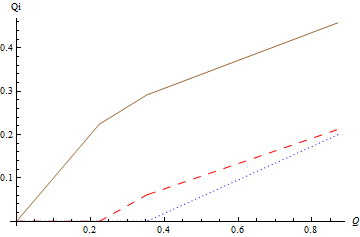
\includegraphics[height=4 cm]{3.png} \\

\end{array}%
$%
\caption{Q vs Qi for all iterations with $Q_3$, $Q_1$, $Q_2$ from top to bottom}
\label{fig:Graphs}
\end{figure}
\end{frame}
\begin{frame}{Continuity}
It is worthwile to demonstrate the continuity of our solutions for the $Q_i$'s.  To do this we need to show that the optimal solutions match at the boundaries where a subspace is discarded. Hence we want to show

\[Q^{(n)}_i (Q=Q^{(n)N-n}_c) = Q^{(n+1)}_i (Q=Q^{(n)N-n}_c)\]

Where we have chosen to consider the $n$th iteration of the solution and now have decided to discard the $N-n$th subspace. 
\end{frame}
\begin{frame}
 Now the equality we want to demonstrate is
\[ \frac{Q_{0,i}\Lambda_{N-n} - \omega_i F_{N-n}+Q^{(n)N-n}(\omega_i-Q_{0,i})}{\Lambda_{N-n} - F_{N_n}} =\]
\[=\frac{Q_{0,i}\Lambda_{N-n-1} - \omega_i F_{N-n-1}+Q^{(n)N-n}(\omega_i-Q_{0,i})}{\Lambda_{N-n-1} - F_{N_n-1}} \]

If we multiply through by the denominators, group and eliminate like terms we get

\[F_{N-n}\Lambda_{N-n-1} - \Lambda_{N-n}F_{N-n-1} + Q^{(n)N-n}_c[\omega_{N-n} - Q_{0,N-n}] = 0\]

\end{frame}
%%%%%%%%%%%%%%%%%%%%%%%%%%%%%%%%%%%%%%%%%%%%%%%%%%%
%%%%%%%%%%%%%%%%%%%%%%%%%%%%%%%%%%%%%%%%%%%%%%%%%%%%%

\begin{frame}{Failure Rate Intersection}

The question of whether the failure rates can intersect is interesting and deserves some attention.  Let us start discussing it in the context of two subspaces.  We realize that if $Q_{0,1} >  Q_{0,2}$ and $Q^1_c < Q^2_c$ then the values of the failure rates never coincide.  The second inequality can be restated thusly:

\[\frac{Q_0 - \bar{Q_{0,1}}}{1- \bar{Q_{0,1}}} < \frac{Q_0 -\bar{Q_{0,2}}}{1-\bar{Q_{0,2}}}\]
Multiplying thorugh and simplifying we find this equals
\[Q_0(\bar{Q_{0,1}}- \bar{Q_{0,2}})<(\bar{Q_{0,1}}- \bar{Q_{0,2}})\]
This equality holds if
\[\bar{Q_{0,1}}> \bar{Q_{0,2}}\]
\end{frame}
\begin{frame}
Unfortunately this does not prove the desired first inequality.  In fact, it is possible to construct a counterexample by these two conditions.  Specifically, if we choose $cos \theta_1 = \frac{1}{4}$ and $cos \theta_2 = \frac{1}{2}$, $\eta_1 = \eta_2$, $r_1 = s_1 \frac{3}{4}$, $r_2 = s_2 = \frac{1}{4}$, we find that $Q_{0,1} = \frac{\sqrt{3}}{16}$ and $Q_{0,2} = \frac{1}{8}$.  With these values we find $Q^1_c \approx .1$ and $Q^2_c <0$:

\begin{figure}[th]
\centering
$%
\begin{array}{c}
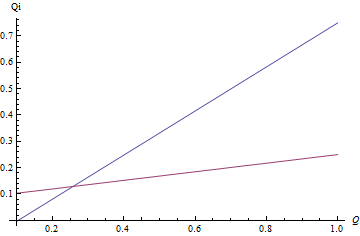
\includegraphics[height=4 cm]{FailureIntersect.png} \\

\end{array}%
$%
\caption{Q vs Qi with Q1 starting higher and going to the origin}
\label{fig:Graphs}
\end{figure}
\end{frame}
\begin{frame}

If there are more than two subspaces, we can generalize this idea:  assume $Q_{0,i} > Q_{0,j}$ and find that for $Q^i_c < Q^{j}_c$ we need $\bar{Q_{0,i}}> \bar{Q_{0,j}}$.  Furthermore, we can consider what happens at later critical points: Since \[Q^{(n)i}_c = \frac{ \omega_{i} F_{N-n} -  Q_{0,i}\Lambda_{N-n}}{\omega_i - Q_{0,i}}\]

then the condition for $Q^{(n)i}_c < Q^{(n)j}_c$ we find the requisite inequality to be

\[\Lambda_{N-n} (\bar{Q_{0,i}} - \bar{Q_{0,j}})> F_{N-n} (\bar{Q_{0,i}} - \bar{Q_{0,j}})\]

which is clearly satisfied by the same requirement as the first critical point.  This creates a structure on the intersection of failure rates:  if $Q_{0,i} > Q_{0,j}$ and $\bar{Q_{0,i}} \leq \bar{Q_{0,j}}$, the two failure rates $Q_i$ and $Q_j$ will intersect at some iteration.
\end{frame}
%%%%%%%%%%%%%%%%%%%%%%%%%%%%%%%%%%%%%%%%%%%%%%%%%%%%%%%%%%
%%%%%%%%%%%%%%%%%%%%%%%%%%%%%%%%%%%%%%%%%%%%%%%%5
\begin{frame}{Single-State Domain}
Each subspace failure rate also has a ceiling.  For the majority of initial conditions the UD failure rate $Q_{0,i}$ sets this upper bound.  For the other cases, we find it from the constraint that $\Pi_{0,i} \leq \vert 0 \rangle_{ii} \langle 0 \vert $.  The equality limit is a full projector which eliminates another measurement and moves us from the POVM to the single-state domain (SSD).
\end{frame}
\begin{frame}
For the single subspace case the equation for the critical ceiling was
\[ Q = Q_c = \frac{2\eta_1\eta_2 sin^2 \theta}{1-Q_0}\]

This result was derived from the constraint that $\xi \leq 1$ where $ \Pi_0 = \xi \vert 0 \rangle \langle 0 \vert$.  Evaluating $\xi$ for the optimal solution gave us 

\[ \xi \leq \frac{1-Q_0}{sin^2 \theta} \frac{Q_0}{2 \eta_1 \eta_2}\]

 where we take the equality limit and set $\xi = 1$ to find the region in which the POVM strategy outperforms the projector measurement. 
\end{frame}
\begin{frame}
There are two regions that this occurs. 
\begin{itemize}
\item
For $\eta_1 \geq \eta_2$, the SSD overlaps with the interpolation measurement in the region $\frac{1}{1 + cos^2 \theta} \leq \eta_1$ and when $Q \geq Q_c$.  

\item
For $\eta_2 \geq \eta_1$ this happens when $\frac{cos^2 \theta}{1+cos^2\theta} \geq \eta_1$ and  $Q \geq Q_c$. 
\end{itemize}
 Because the failure operator points directly onto the less likely state in either of these cases, we find the failure rates to be simply $Q^<= \eta_2 + \eta_1 cos^2 \theta$ and $Q^> = \eta_1 + \eta_2 cos^2 \theta$ respectively. 
\end{frame}
\begin{frame}
To generalize to subspaces we return to the bar normalization that renormalized the subspace probabilities to 1.  Remembering that

\[Q_i =  \xi_i \langle 0_i \vert D_i \vert 0_i \rangle\]

where $D_i$ is the full density matrix of the states in the $i$th subspace, $ D_i = \eta_{1,i} \rho_{1,i} + \eta_{2,i} \rho_{2,i}$ we can conclude that 

\[ \bar{Q_i} = \xi_i \langle 0_i \vert \bar{D_i} \vert 0_i \rangle\] 

where $\bar{D_i} = \bar{\eta_{1,i}} \rho_{1,i} + \bar{\eta_{2,i}} \rho_{2,i}$
\end{frame}
\begin{frame}
Now we have restored the summation of the a-priori probabilities for each subspace to 1 while leaving $\xi_i$ unchanged, so the preceding arguments for the single subspace can be implemented to rewrite the inequality for $\xi_i$ as 

\[ \xi_i \leq \frac{1-2\sqrt{\bar{\eta_{1,i}} \bar{\eta_{2,i}}} cos \theta_i}{1-cos^2 \theta_i} \frac{cos\theta_i}{\sqrt{\bar{\eta_{1,i}} \bar{\eta_{2,i}}}}\]

or

\[ \xi_i \leq \frac{\omega_i-2\sqrt{\eta_{1,i} \eta_{2,i}} cos \theta_i}{1-cos^2 \theta_i} \frac{cos\theta_i}{\sqrt{\eta_{1,i}\eta_{2,i}}}\]
\end{frame}
\begin{frame}

 we get the natural generalization of the critical ceiling to subspaces to be
\[ Q_i = Q^{cc}_i =\frac{2\eta_{1,i} \eta_{2,i} sin^2 \theta_i }{\omega_i-Q_{0,i}}\] 

As $Q_i$ is increased past this point we have  $\Pi_{1,i} = \vert 1 \rangle_{ii} \langle 1 \vert $ and $\Pi_{0,i} = \vert 0 \rangle_{ii} \langle 0 \vert $ 
\end{frame}
\begin{frame}
 Now the condition for the overlap of the SSD onto the POVM region,  assuming $\eta_{1,i} \geq \eta_{2,i}$ is

 \[\frac{\omega_i}{1+cos^2 \theta_i} \leq \eta_{1,i}\]

With the maximum failure rate that can be generalized as: $Q^{<}_i = \eta_{2,i} + \eta_{1,i} cos^2 \theta_i$

Similarly for $\eta_{2,i} \geq \eta_{1,i}$ we get the condition 

 \[\frac{\omega_i cos^2 \theta_i}{1+cos^2 \theta_i} \geq \eta_{1,i}\]

and the maximum failure rate as  $Q^{>}_i = \eta_{2,i} + \eta_{1,i} cos^2 \theta_i$

\end{frame}

\begin{frame}

We notice that with more subspaces, the condition for the overlap region of SSD over the POVM does not change for individual subspaces as the bar transformation would show us.

We show these elements in the following figure, where the shaded regions represents the SSD domains.
\end{frame}
\begin{frame}
\begin{figure}[th]
\centering
$%
\begin{array}{c}
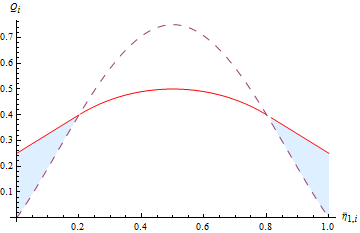
\includegraphics[height=4 cm]{SSD.png} \\

\end{array}%
$%
\caption{ $\bar\eta_{1,i}$ vs $Q_i$  The dashed line represents $Q_i^{cc}$ and the sold line the absolute maximum $Q_i$, the intersection point of the two is determined by the inequalities above.  Values given for $\theta_i = \pi /3$ }
\label{fig:Graphs}
\end{figure}
\end{frame}
\iffalse
\begin{frame}{Examples}
It is worthwhile to show a numerical example of this method in detail.  We consider three subspaces with $\eta_1 = \eta_2$ and these parameters:

Subspace 1 has:  $r_1 = 1/4$, $s_1 = 1/4$ and  $\theta_1 = \frac{\pi}{4}$ so that $\omega_1=1/4$ and its maximum failure rate is $Q_{0,1} = \sqrt{2}/8 \approx .17$

Subspace 2 has:  $r_2 = 3/8$, $s_2 = 1/8$ and $\theta_2 = \frac{\pi}{4}$ so that $\omega_2=1/4$.  Its maximum failure rate isn't $Q_{0,2} = \sqrt{6}/16 \approx .15$ because it fails one of the SSD conditions and instead $Q^{<}_2 =7/32 \approx .21$ 

Subspace 3 has:  $r_3 = 3/8$, $s_3 = 5/8$ and $\theta_3 = \frac{\pi}{6}$ so tha $\omega_3=1/2$. Its maximum failure rate isn't $Q_{0,3} = 3 \sqrt{5}/16 \approx .42$, because it fails the other SSD condition and instead $Q^{>}_3 = 29/64 \approx .45$

The failure rate maximum $Q^{MAX} = Q_{0,1} +Q^{<}_2 +Q^{>}_3 \approx .87$ while $Q_0 \approx .75$
and $\sum \omega_i = 1$ as it should.
\end{frame}
\begin{frame}{First Elimination}

To find which subspace to discard first we find the critical Q's:

$Q^1_c \approx .146$, $Q^2_c \approx .355$, $Q^3_c <0$, so subspace 2 is discarded first when $Q \approx .355$.  This means that $Q_2 =0$ when $Q = Q^2_c$ and we do not allow the value of $Q_2$ to vary afterward.

At $Q^2_c$ we find the values of the other failure rates to be $Q_1 \approx .05$ and $Q_3 \approx .28$
\end{frame}
\begin{frame}{Second Elimination}

It may be clear that $Q_1$ will reach 0 first and indeed this is so.  Before we find the second set of critial values we find our new constants as:

$\Lambda_2 = \sum^{1,3}\omega_i = 3/4$; $ F_2 = \sum^{1,3} Q_{0,i} \approx .6$

Now the critical values read
$Q^{(1)1}_c \approx .22$ and $Q^{(1)3}_c <0$ so when $ Q = Q^{(1)1}_c$ we discard subspace 1 and reduce the optimization problem to the single subspace case, where $Q^{(2)3} = Q$. This process is depicted in the graph below. 

\end{frame}
\fi

\begin{frame}{Subspaces Summary}
We found several surprising and extraordinary conclusions.  The first is that the form of the error rate remains the same over all subspaces.  The second is the threshold behavior in the optimization that shuts off successive subspaces as the total failure rate decreases.
\end{frame}
%%%%%%%%%%%%%%%%%%%%%%%%%%%%%%%5
%%%%%%%%%%%%%%%%%%%%%%%%%%%%%%%%%%
\section{Future Work}
\subsection{2D Mixed States}
\begin{frame}{2D Mixed States}
A problem we are currently working on is to distinguish between two mixed states in two dimensions. We can represent them as:

\[ \rho_1 = p \ke {\psi_1} \br {\psi_1}  + \frac{(1-p)}{2} I\] 
and
\[ \rho_1 = d \vert \psi_2 \rangle \langle \psi_2 \vert + \frac{(1-d)}{2} I\]

Where the pure states $\vert \psi_1 \rangle = c_1 \vert 0 \rangle + s_1 \vert 1 \rangle $ and $\vert \psi_2 \rangle = c_2 \vert 0 \rangle + s_2 \vert 1 \rangle $ form a 2 dimensional space and p,d are the purities of the two mixed states.

The a-priori probabilities are as usual $\eta_1$ and $\eta_2$
\end{frame}
\begin{frame}
We cannot in general distinguish perfectly between these two because are are not in general orthogonal. We also cannot distinguish them unabmiguously in general because of the identity terms. Hence it is less clear which strategy is better.  An interpolative approach will allow us to see the transition between ME and MC and understand the trade-off in increasing the failure rate for different starting conditions.  We use the transformation discussed earlier to tackle this problem.
\end{frame}
\begin{frame}
We want to implement the transformation that gives us

\[ \td {\rho_1} = \frac{\Omega^{1/2} \rho_1 \Omega^{1/2}}{Tr(\Omega \rho_1)} \]
\[ \td {\eta_1} = \frac{\eta_1 Tr (\Omega \rho_1)}{1-Q}\] 

So that we still have $Tr \td {\rho_1} = 1 $ and $\td {\eta_1 } + \td {\eta_2} = 1$
and the error rate is

\[\td{P_e} = \frac{1}{2}(1 - Tr \abs{\td{\Lambda}})\]
where $\td{\Lambda} = \td{\eta_1}\td{\rho_1} - \td{\eta_2}\td{\rho_2}$
\end{frame}
\begin{frame}
We work on the lambda to find:
\[Tr \abs{\td{\Lambda}} = \frac{1}{1-Q} Tr \abs{\Omega^{1/2}\Lambda \Omega^{1/2}}\]
where $\Omega^{1/2} =  \left( \begin{array}{cc}
\sqrt{1- \xi} & 0 \\
0 & 1 \end{array} \right)$ and

$\Lambda = \left( \begin{array}{cc}
{p\eta_1c_1^2-d\eta_2c_2^2 + \frac{\eta_1(1-p) -\eta_2(1-d)}{2}} &{ p\eta_1c_1s_1-d\eta_2c_2s_2} \\
{p\eta_1c_1s_1-d\eta_2c_2s_2} & {p\eta_1s_1^2-d\eta_2s_2^2 + \frac{\eta_1(1-p) -\eta_2(1-d)}{2}}\end{array} \right)$ 

\end{frame}
\begin{frame}

$\Omega^{1/2}\Lambda \Omega^{1/2} = \td {\Lambda}$ is easy to find 

To find the sum of the absolute values of its eigenvalues we first write the characteristic equation as

\[ \lambda^2 - b \lambda + c = 0\]

where

\[b = \eta_1 -\eta_2 - \xi [ p\eta_1 c_1^2 - d\eta_2 c_2^2 + \frac{\eta_1(1-p) - \eta_2(1-d)}{2}]\]
and
\[c = (1-\xi)[ \frac{1- 4\eta_1\eta_2 -(p\eta_1 -d \eta_2)^2}{4} -pd \eta_1\eta_2 (c_1s_2-c_2s_1)^2]\]

Where we can rewrite the term $ (c_1s_2-c_2s_1)^2 = sin^2 \theta$ 
\end{frame}
\begin{frame}
We can find $\xi$ by solving


\[1-Q = Tr \Omega \rho = 1- \xi [ p\eta_1 c_1^2+ d\eta_2 c_2^2+ \frac{1-p\eta_1 -d\eta_2}{2}]\]

We can solve the quadratic equation $\lambda^2 -b \lambda +c$ for the two eigenvalues, but we notice that for $p=d=1$ the value of c is $c= (1-\xi)[-\eta_1\eta_2 sin^2 \theta]$ is negative and for $p=d=0$ the value of c is $c= (1-\xi)[\frac{(\eta_1-\eta_2)^2}{4}]$ is positive. 

 Hence the sum of the eigenvalues for $c<0$ is

\[\sum \abs {\lambda_i} = \sqrt{b^2-4c}\]

And the sum of the eigenvalues for $c \geq 0$ is

\[\sum \abs {\lambda_i} =b\]

\end{frame}
\begin{frame}
As we noted before, this is not the final solution.  A further optimization is required to determine $c_1$ and $c_2$.  Considering the complexity of the b and c terms, this is not trivial.  We hope to be able to solve at least some of the specific cases if not for all of them.  Simpler cases include $p=d$, when the purity of both states are equal.  Another is $d=1$, where we discriminate between one pure and one mixed state.
\end{frame}
\section*{Summary}

\begin{frame}{Summary}

  % Keep the summary *very short*.
  \begin{itemize}
  \item
    The \alert{first main message} of your talk in one or two lines.
  \item
    The \alert{second main message} of your talk in one or two lines.
  \item
    Perhaps a \alert{third message}, but not more than that.
  \end{itemize}
  
  % The following outlook is optional.
  \vskip0pt plus.5fill
  \begin{itemize}
  \item
    Outlook
    \begin{itemize}
    \item
      Something you haven't solved.
    \item
      Something else you haven't solved.
    \end{itemize}
  \end{itemize}
\end{frame}



% All of the following is optional and typically not needed. 
\appendix
\section<presentation>*{\appendixname}
\subsection<presentation>*{For Further Reading}

\begin{frame}[allowframebreaks]
  \frametitle<presentation>{For Further Reading}
    
  \begin{thebibliography}{10}
    
  \beamertemplatebookbibitems
  % Start with overview books.

  \bibitem{Author1990}
    A.~Author.
    \newblock {\em Handbook of Everything}.
    \newblock Some Press, 1990.
 
    
  \beamertemplatearticlebibitems
  % Followed by interesting articles. Keep the list short. 

  \bibitem{Someone2000}
    S.~Someone.
    \newblock On this and that.
    \newblock {\em Journal of This and That}, 2(1):50--100,
    2000.
  \end{thebibliography}
\end{frame}

\end{document}


